\chapter{Linear Projection}
\label{chapter:projection}

We would like to define a region of interest that contains only one uni-model for exploitation.
Also, some algorithms, e.g. SPSO, requires a well-defined hypercube search space with fixed-value constraints in each dimension.
Defining the projection onto subspace can be described as a model selection.
In our case, this process does not require high accuracy, yet has a strict demand on time consumption.
Combining the requirements, we use a linear projection matrix to project the original search space 
onto a subspace with feasible solutions bounded within $[0,1]$ in each dimension.

One of the advantage for using projection matrix is that for a problem with $\ell$ variables, 
a linear projection matrix on homogeneous coordinate only requires $(\ell+1)^2$ hyperparameters to be optimized.
Therefore, less hyperparameters are assigned than directly define each hyperplane borders or vertices.  
This reduces the parameters that we need to optimize and results in less time consumption during model selection.
We also use the (1+1)-ES, a fast and simple evolutionary strategy, to optimize the matrix.
It allows us to rapidly approximate a high dimensional projection matrix within given number of iterations.

Furthermore, subspace projection also gives advantage for solving \textit{inseparable problems}.
For variabels that are not independent, projection allows the algorithm
to solve an easier, rotated and sheared problem on subspace, as shown in Figure~\ref{fig:Projected_ROI}.
The homogeneous projection matrix seperates the original ROI into less overlapped ROI, 
which reduces redundant search and sometimes enlarges the crutial regions.

In the following sections, we first describe the cannonical affine transformation.
Then we discuss how the projection matrix allows linear projection in a homogeneous coordinate.
Finally, we give details of how we design the cost function and how we utilize the (1+1)-ES to optimize the projection matrix.

\begin{figure}
\centering
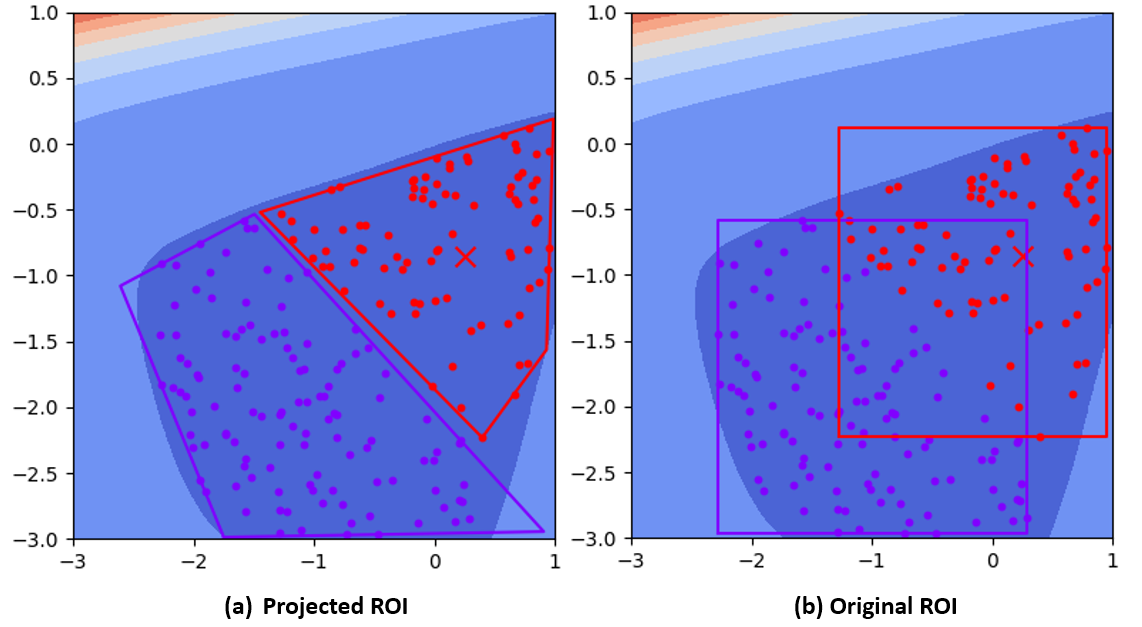
\includegraphics[width=\textwidth]{Projected_ROI}
\caption{Projecting inseparable problems onto subspace.}\label{fig:Projected_ROI}
\end{figure}



\section{Affine Transformation}
In geometry, an affine transformation preserves points, straight lines and planes.
For two affine spaces $A$ and $B$ and any pair of points $P, Q \in A$,
an affine transformation $f$ determines a linear transformation $\varphi$ that can formally defined as:
\begin{displaymath}
\overrightarrow{f(P)f(Q)} = \varphi \overrightarrow{(PQ)}
\end{displaymath}

In the following paragraph, we list some common affine transformation matrix in 2D.
\begin{enumerate}
    \item Translation 
            
            Translation moves every point in the cluster by the same amount in a given direction.
            It allows us to reallocate the center of ROI.

\begin{figure}[H]
\centering
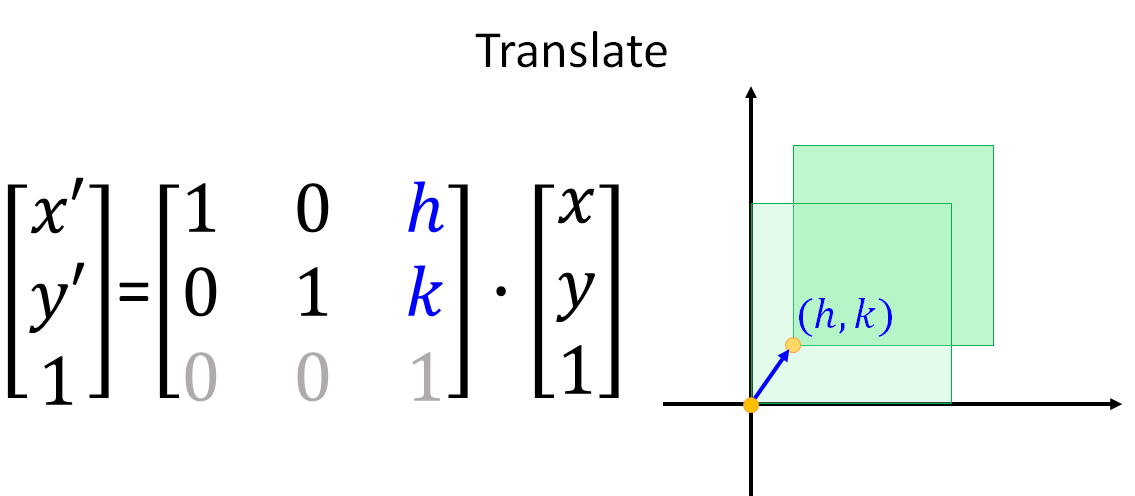
\includegraphics[width=\textwidth]{Translation}
\caption{Translation in 2D}\label{fig:Translation}
\end{figure}


    \item Rotation 

\begin{figure}[H]
\centering
%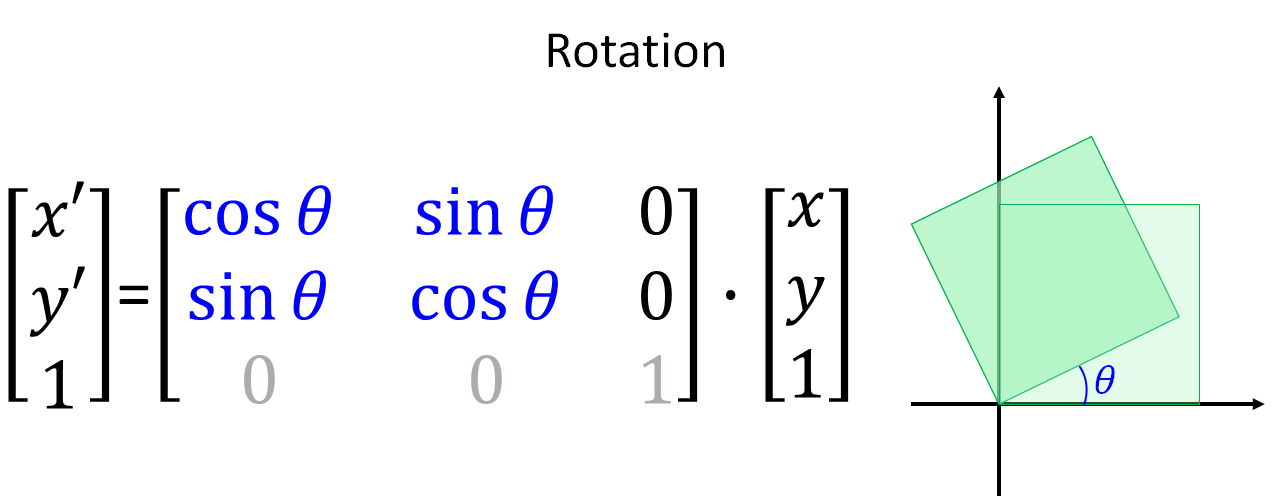
\includegraphics[width=\textwidth]{Rotation}
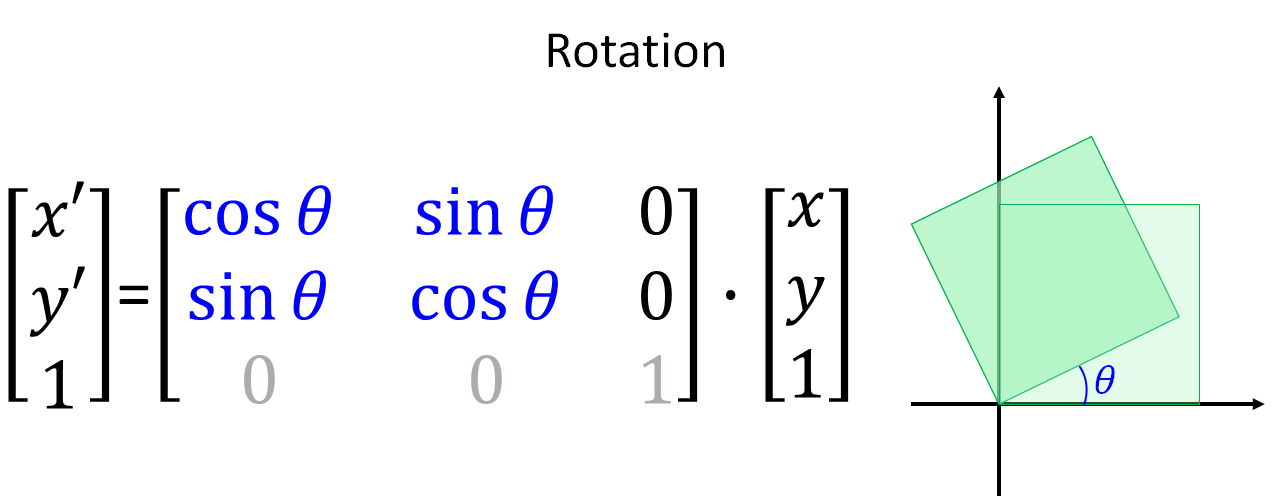
\includegraphics[]{Rotation}
\caption{Rotation in 2D}\label{fig:Rotation}
\end{figure}

    \item Scaling 

\begin{figure}[H]
\centering
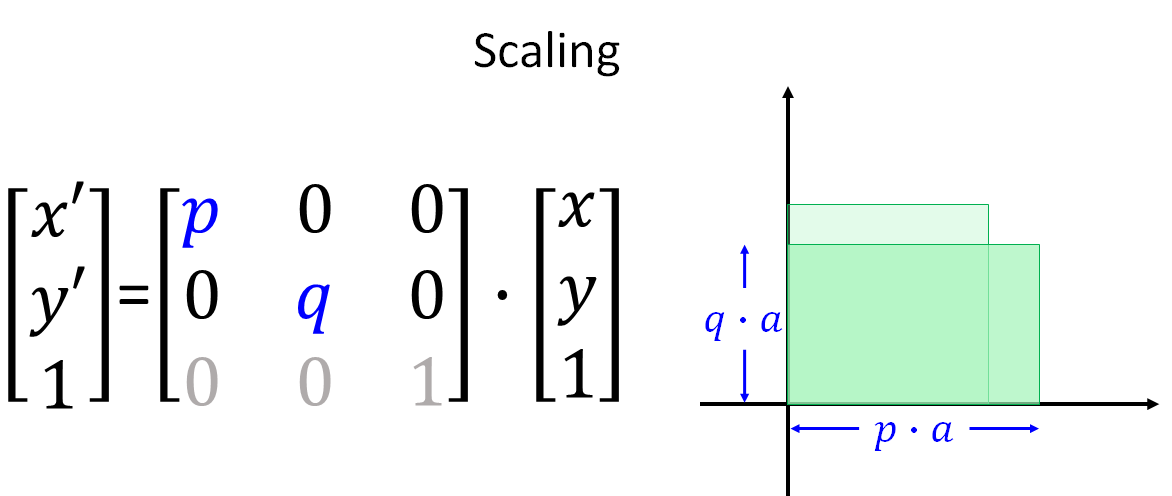
\includegraphics[width=\textwidth]{Scaling}
\caption{Scaling in 2D}\label{fig:Scaling}
\end{figure}

    \item Shearing 

\begin{figure}[H]
\centering
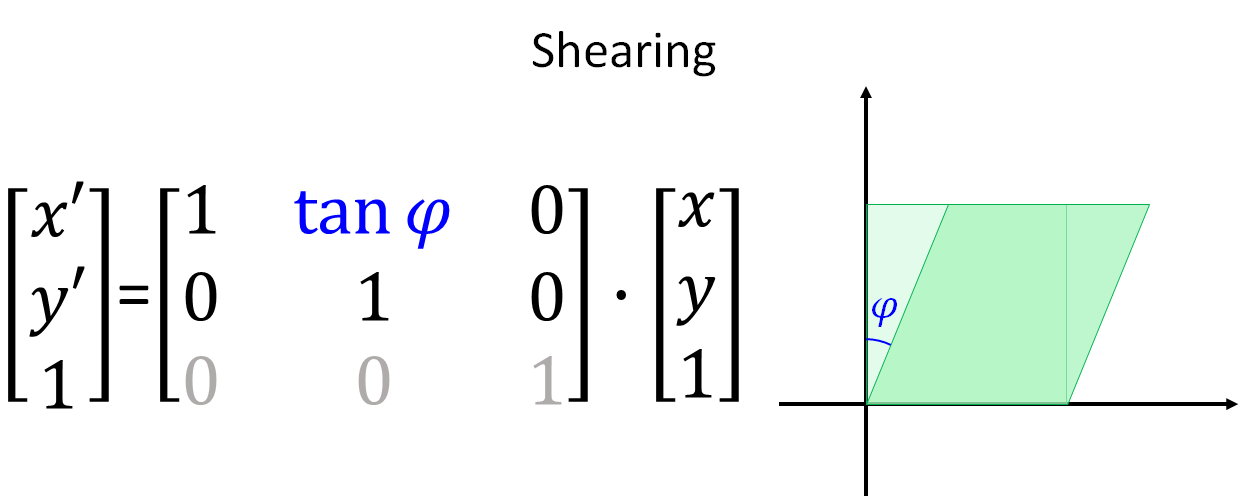
\includegraphics[width=\textwidth]{Shearing}
\caption{Shearing in 2D}\label{fig:Shearing}
\end{figure}

\end{enumerate} 


General affine transformation

\begin{figure}[H]
\centering
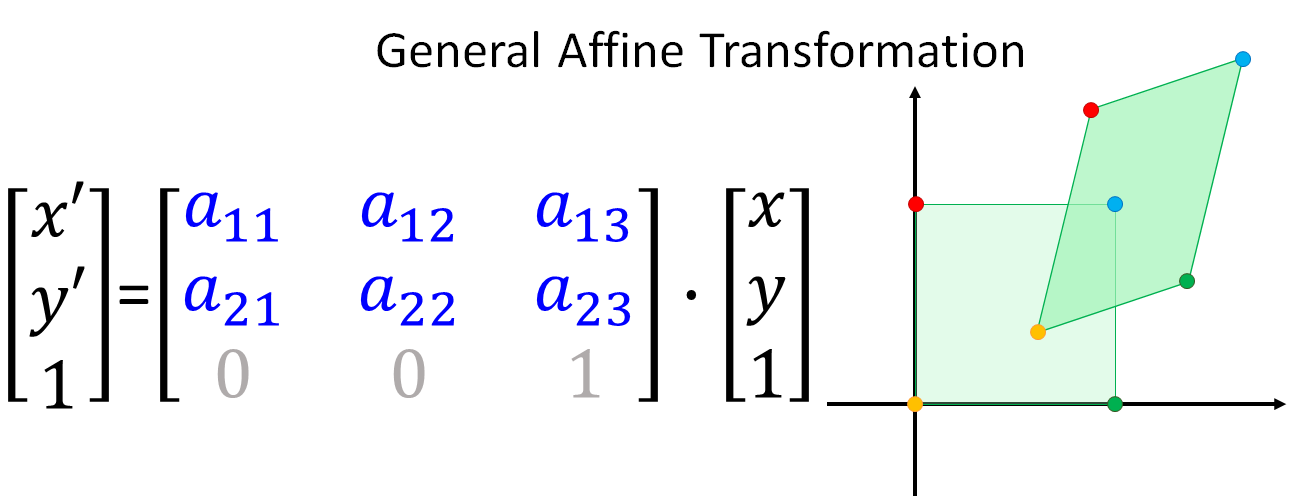
\includegraphics[width=\textwidth]{Affine}
\caption{General affine transformation in 2D}\label{fig:Affine}
\end{figure}





\section{Projective Transformation}

Projective transformations are the most general linear transformations and require the use of homogeneous coordinates.
Homogeneous coorinate is ...

Augmented Matrix

Finally, \textit{recover} the projected point using \textit{homogeneous convention}, 
On a $d$-dimensional space, we convert the projected position, a vector with $(d+1)$ variables, to a $d$ variable vector 
by dividing first $d$ elements with the last element.

\begin{figure}
\centering
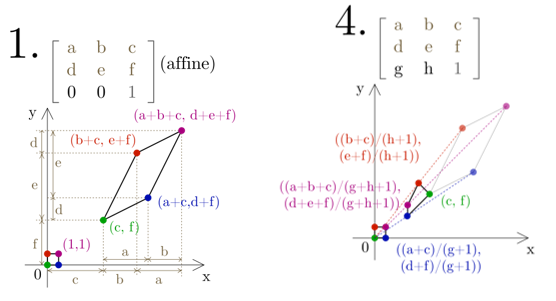
\includegraphics[width=\textwidth]{Affine_vs_Projective}
\caption{Affine transformation and projective transformation comparison.}\label{fig:Affine_vs_Projective}
\end{figure}









\section{Optimization for Projection Matrix}

After identifying different clusters of samples, which represents a uni-modal, 
we would like to further define a reasonably good ROI.
In order to obtain a nice ROI for a problem with $D$ variables, 
we need to optimize the $(D+1)^2$ parameters in the projection matrix with a loss function.
The loss function should cost little computational time and should suggest the right direction for optimization, 
in order to match the restrictions of a well-defined ROI.
Also, the optimization only needs to define a reasonably well ROI for the alogirthms to search.  
In the later iterations, the matrix update procedure allows us to define a more accurate ROI with a better insight of the uni-modal subproblem.
In our case, it is acceptable to sacrefice a bit of accuracy for computational time in hyperparameters tuning.  
We will describe the desgin of our loss function and the advantage of using a (1+1)-ES to optimize the matrix in the following sections.  


\subsection{Loss function}

The goal of the ROI is to seperate the search space into non-overlapping subspaces, 
each containing an approximately normalized fitness hill.
In our loss function, we considered the following features:
\begin{enumerate}
    \item Distances to the boundary for the \textbf{points within the cluster} yet excluded in the ROI.
    \item Distances to the boundary for the \textbf{random samples within other ROIs} yet included in the ROI.
    \item Distances to the boundary for the \textbf{random samples} in the subspace that are outside of the original search space boundary.
    \item Distance of the weighted \textbf{mean} to the center of subspace $[0.5]^D$
    \item The Mean Absolute Error (MAE) for each element in the weighted \textbf{covariance matrix} to a scaled identicle matrix
    \item The sum of \textbf{reconstruction} error for each particle 
\end{enumerate} 
We add up all the errors mentioned above and try to minimize that error. 
Following part explains the reason for considering each features.

First, we would like to keep all the particles that belong to this cluster in the boundary $[0,1]^D$.
It can easily be done by projecting all points within the cluster onto the subspace, 
and check whether if any of the projected position is outside of the boundary $[0,1]^D$.

Second, we would like to avoid ROIs from overlapping by adopting the Monte Carlo method for region collision detection. 
When optimizing one ROI, we randomly generate a given amount of samples within the subspace for all the other ROIs.
Then, we use the inverse projection matrix of each other ROIs to project these sample points back to the original search space.
After that, we use the projection matrix of the ROI that we are optimizing to project all the exterior samples onto the subspace.
This way, we can easily discover which exterior samples are within the $[0, 1]^D$ boundary.
Figure~\ref{fig:Sample_projection} shows a screen shot of the red ROI before and after optimizing the projection matrix of the red ROI.
We randomly generates 200 samples within the green and blue ROI and tries to exclude them in the red ROI.

\begin{figure}
\centering
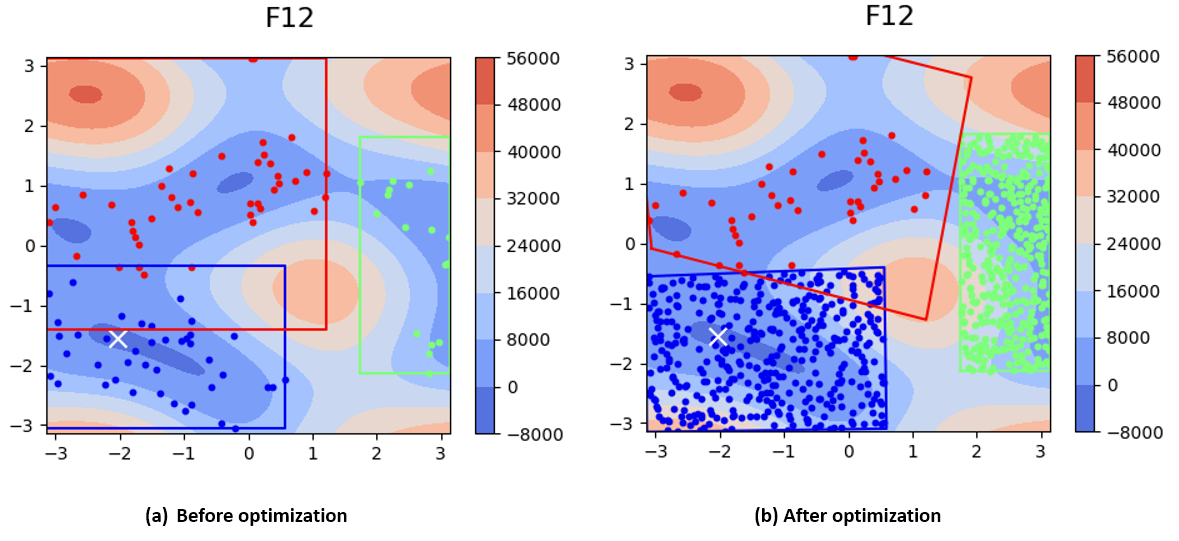
\includegraphics[width=\textwidth]{Sample_projection}
\caption{Optimization of projection matrix.}\label{fig:Sample_projection}
\end{figure}

Third, we also use the Monte Carlo method described before to make sure that the ROI does not exceed the boundaries of the orignal subspace.
We randomly generate samples from the subspace and inverse project it back to the search space to make sure that all points are within boundaries.
If not, we would like to minimize the distance of sample points to the nearest border.

Forth, we would also like each underlying model for each subproblem 
to be a multivariate gaussian distribution with mean around the center $[0.5]^D$.
If the algorithm searches near the boundary, it indicates that ROI should be updated since the optimum solution might be outside of the border.
Placing the optimum solution at the center of the search space creates a more stable model for the algorithm to search.
This allows a thorough search around the center, and decreases the frequency of ROI update.
Therefore, we calculate the weighted mean of the points within the cluster on the subspace.
Then we minimize the distance of weighted mean to the center.  

Fifth, we would like the weighted covariance matrix to be approximately $0.2I$, where $I$ is an identicle matrix.
This enables the projection matrix to rotate, scale, and shear a fitness hill.
The normalization preprocess is a common technique to make future optimization easier.
Therefore, we calculate the MAE between the weighted covariance matrix and $0.2I$.  

Finally, since the we project the particle positions in a homogeneous coordinate,
the correlations between reconstructed positions on the subspace might not be identical to the original ones.
We would like to minimize the transformation error while keeping the ROI within the original boundaries.
Therefore, for each possible matrix solutoin, we use it to project all points in the corresponding cluster onto a subsapce.
Later, we use the inverse matrix to project all the points back to the original search space to get the reconstructed positions.
Then, we calculate the MAE of all points in all dimensions between the original position and the reconstructed positions.


%Given a possible solution of the projection matrix $X = [x_1, x_2, ..., x_{(d+1)^2}]$ for a problem with $d$ variables.
%Let the corresponding projection matrix be $\textbf{A}$ with shape $(d+1) \times (d+1)$.
%We define the linear projection mapping any position $\vec{x}$ to the subspace as $T$, then
%\begin{displaymath}
%T(\vec{x}) = \textbf{A}\vec{x} 
%\end{displaymath}


%matrix $A$, we define the loss function $f$ as: 

%\begin{align*}
%f(X)                &= D_{include} + D_{exclude} + D_{boundary} + D_{center} + D_{covariance} + D_{reconstruction} \\ D_{include}         &= \\
%D_{exclude}         &= \\ 
%D_{boundary}        &= \\ 
%D_{center}          &= \\ 
%D_{covariance}      &= \\ 
%D_{reconstruction}  &= \\ 
%\end{align*}


\subsection{Optimization Algorithms}

With the loss function defined in the previous section, 
we still need an optimization algorithm to optimize the projection matrix.
The difficulty for \textit{hyperparameters optimization} is to balance between speed and optimization ability.
We need the hyperparameters to define a subspace that contains the possible optimum solution while costing few computation time.

We can simplify and stablelize the optimization process by giving a fixed initial solution.
Here, the initial solution is a simple dot product of a translation matrix and a scaling matrix. 
The matrix defines a hypercube, which is bounded by the minimum and maximum value in each dimension of all positions in the cluster.
This allows the algorithm to start the search around a more prefered neighborhood.

We first tried to use CMA-ES.

Later, we utilize the (1+1)-ES, described in Algorithm~\ref{algo:1+1ES}.

Finally, we did an approximation for the infeasible solutions that belong to the cluster yet being outside of ROI after the optimization.
We normalize the distance between the infeasible solution and the center of ROI,
to project it onto a hypershpere centering at $[0.5]^D$ and with radias $0.5$.
This way, although the reconstructed position is not accurate on the original search space,
it is still able to indicate the approximate fitness in that direction in the subspace.
Also, our basic assumption is a unimodal hill that puts the best fitness point in the center.
Therefore, marginal points should have lower fitness and should not spend more resources to exploit.
It just needs to give us a hint of the gradient in that direction.
